driv
%\chapter{Školy}\label{Skoly}
\chapter{Simulace opatření ve školním prostředí}\label{Skoly}

\textit{Tomáš Diviák, Jakub Drbohlav}
\vspace{15mm}

\section*{Úvod\footnote{Tato kapitola vychází z modelu, který autoři vypracovali v souvislosti s nastavováním režimových opatření v českých školách. Kompletní výsledky modelu jsou shrnuty v článku, o jehož publikaci autoři usilují v zahraničních epidemiologických časopisech, částečné výsledky byly rovněž shrnuty ve výzkumné zprávě na webu BISOP (BISOP 2021, \url{https://www.bisop.eu/vyzkumna-zpravabisop-vytvoril-model-sireni-covidu-19-na-zakladnich-skolach/}).}}

Podobně jako jiné infekční choroby, i covid-19 se šíří prostřednictvím relevantních kontaktů mezi lidmi, při nichž dochází k přenosu viru \cite{pg:kucharski2020, vespignani2020modelling}. To se může dít v mnoha prostředích lidské aktivity od rodin, přes nákupy až po pracoviště. Jedním z takových prostředí, kde se covid-19 a také další respirační onemocnění šíří, jsou i školy. Uzavírání škol patřilo po celém světě mezi první protiepidemická opatření ve snaze co nejrychleji a nejefektivněji zamezit prudkému nárůstu počtu nově nakažených jedinců v celé populaci. Od poloviny března loňského roku tak školy v Česku fungovaly v různou měrou omezeném režimu a i v květnu 2021 stále trvají některá omezení výuky.

I přes určitou míru nejistoty panuje mezi vědci konsenzus na tom, že školy patří mezi prostředí, v nichž je riziko nákazy a následného přenosu mimo ni relativně vysoké a že uzavírání škol patří mezi jedno z nejefektivnějších opatření pro omezení šíření covid-19 \cite{Brauner_etal2020, lessler2021household, Haug_etal2020}. Dlouhodobé uzavření škol má ale také významné negativní dopady na žáky a studenty i učitele. Mezi tyto negativní dopady patří nízká efektivita distanční výuky s ohledem na vzdělávací výsledky dětí \cite{engzell2021learning}, ale také psychické a sociální dopady způsobené nedostatkem interakcí s vrstevníky \cite{bignardi2020longitudinal, ravens2021impact} a v rovině ekonomické pak také náklady plynoucí z toho, že jsou rodiče s dětmi doma namísto práce. Někteří odborníci dokonce upozorňují, že dlouhodobé dopady uzavření škol mohou navíc disproporčně více dopadnout na děti ze sociálně znevýhodněných rodin \cite{di2020likely}.

Zmírnění epidemie za cenu omezení vzdělávacích a socializačních funkcí škol tak představuje určité dilema, s nímž se potýká veškeré uvažování o tom, za jakých podmínek školy uzavírat či znovuotevírat během pandemie. Modelování a simulace založené na datech přestavují v tomto ohledu možnost, jak toto dilema alespoň částečně vyřešit \cite{squazzoni2020computational}, neboť alternativy v podobě observačních dat buď nejsou dostupné nebo v případě experimentů krajně neetické. Modely pro šíření infekčních chorob tak lze chápat jako jakousi „virtuální laboratoř“ \cite{Rao_etal2021}, v níž lze zkoumat efekty různých opatření a různých vlastností daného patogenu na rychlost a rozsah výsledné epidemie.

Významným podkladem pro modelování a simulace šíření respiračních i dalších infekčních chorob jsou data o sítích kontaktů mezi členy dané populace \cite{danon2011networks, luke2007network, zaj:mossong2008social}. Taková síť je tvořená uzly (v epidemiologickém kontextu zpravidla lidmi) a vazbami mezi nimi, které reprezentují právě tyto kontakty mezi nimi. Tato kapitola se zabývá tím, jak sestrojit síť kontaktů relevantních pro přenos viru SARS-Cov-2 uvnitř jedné konkrétní základní školy a jak následně tuto síť využít při simulaci šíření nákazy a vlivu různých protiepidemických opatření na ni. 


\section*{Data} 
Pro smysluplné modelování potenciálního průběhu epidemie covid-19 na školách je nutné mít adekvátní data. Tato data by měla vypovídat o kontaktech relevantních pro přenos nákazy mezi důležitými aktéry uvnitř školy jako sociálního systému. Za nejdůležitější lze považovat dvě množiny aktérů (uzlů) – žáky a učitele, přičemž kontakty mezi žáky a učiteli, mezi žáky navzájem a mezi učiteli navzájem definují různé úrovně vazeb v síti (grafu). Jednotlivé uzly lze popsat relevantními atributy, u žáků např. předměty, podle nichž je lze seskupovat (cizí jazyky atd.), a příslušnost do jednotlivých tříd, u učitelů pak např. jejich aprobace či věk. 

Typickou školu si lze v tomto ohledu představit jako tzv. víceúrovňovou vícevrstvou síť či graf, v níž figurují dvě úrovně uzlů (bodů v obrázcích 1 a 2) reprezentující dvě hlavní skupiny jedinců uvnitř školy – učitele a žáky. Mezi učiteli i mezi žáky probíhají pro přenos nákazy potenciálně rizikové kontakty znázorněné jako vazby (spojnice mezi uzly v obrázcích 1 a 2). Obrázek 1 zobrazuje všechny učitele a vazby mezi nimi. Vazby relevantní pro přenos viru SARS-Cov-2 mezi učiteli jsou trojího typu: kontakty v kabinetu, v práci mimo kabinet a mimo práci resp. školu. Obrázek 2 potom zobrazuje všechny žáky a vazby mezi nimi, kterých lze rozlišit celkem pět typů vzhledem k přenosu viru SARS-Cov-2. Jedná se o kontakty v lavici, při obědě, během přestávky, ve školní družině a mimo školu. Učitelé a žáci jsou vzájemně propojeni prostřednictvím vazeb výuky, kde má každý učitel vazbu na všechny žáky, které vyučuje, o intenzitě odpovídající počtu vyučovaných hodin a počtu žáků v dané třídě (tato úroveň zde není zobrazena).

Empirická data, která by umožnila sestavit takovouto víceúrovňovou vícevrstvou síť, lze získat v zásadě třemi způsoby. Jedná se o pozorování, simulaci a dotazování. Pozorování v tomto kontextu znamená jakýkoliv způsob, který umožní externím výzkumníkům zjistit, kdo je s kým v rámci zkoumané školy v kontaktu. Jedním ze způsobů, jak takové pozorování provést, je pomocí nositelných snímačů, které dostanou všichni sledovaní aktéři, aby je dobu pozorování nosili (viz např. \cite{stehle2011high, gemmetto2014mitigation}. Tyto senzory elektronicky zaznamenávají, zda a jak dlouho jsou v předem určené blízkosti k ostatním senzorům, tj. jejich nositelům. Výhodami tohoto typu sběru dat jsou přesnost a relativní objektivita takto získaných dat, protože u tohoto způsobu sběru dat lze flexibilně nastavit měření různé délky a vzdálenosti kontaktů a netřeba při tom spoléhat na subjektivní vnímání zkoumaných osob. Nevýhodami pozorovacích technik naopak jsou jejich technické, finanční a časové nároky. Simulace realistických dat na základě známých parametrů a charakteristik odpovídajících sítím, které jsou předmětem zájmu, představuje alternativu, kterou lze také za určitých podmínek použít (viz např. \cite{mcgee2021model, potter2012estimating}. Simulace dat nahrazuje jejich sběr, takže odpadají komplikace spojené s logistickými a finančními nároky sběru dat. To má ale svou cenu v tom, že validita nasimulovaných dat předpokládá dostatečné znalosti o struktuře a dynamice daných sítí, které ne vždy mohou být k dispozici nebo zachycovat všechny podstatné rysy simulovaných sítí.

Posledním způsobem, jak potřebná data získat, je dotazování, z nějž vychází i výsledky ve zbytku této kapitoly. Dotazování představuje pomyslný standard pro sběr dat o lidském chování včetně chování spojeného se zdravím (srv. \cite{danon2011networks, luke2007network, zaj:mossong2008social}. Dobře zkonstruovaný dotazník dokáže získat spolehlivé informace i o velice specifických aspektech chování respondentů. Je nicméně třeba mít na paměti riziko nepřesných odpovědí či neochoty respondentů odpovídat. To vzniká zvláště v případě kognitivně náročných úkonů, mezi něž patří i odpovídání na otázky týkající se typů a četnosti kontaktů a toho, s kým k těmto kontaktům došlo. I proto byl navržený dotazník nakonec maximálně úsporný a dotazoval se jen na ty nezbytně nutné otázky. Aby byla zmapována celá vybraná škola, dotazováni byli všichni učitelé a všichni žáci. Žáci byli dotazováni na kontakty pěti typů (kontakty v lavici, při obědě, během přestávky, ve školní družině a mimo školu) se spolužáky ve své třídě, ale také měli možnost indikovat kontakty s žáky z jiných tříd. Podobně učitelé odpovídali na otázky o kontaktech s ostatními učiteli ve třech situacích (v kabinetu, mimo kabinet ve škole a mimo školu). Pomocí dotazování se také zjistilo, ve kterých třídách jednotliví učitelé vyučují a jak často. Pro usnadnění odpovídání byl respondentům v rámci dotazníku vždy předložen seznam všech dalších žáků (resp. učitelů), v němž měli možnost zvolit, s kým měli daný kontakt. Intenzita kontaktu byla posuzována na čtyřbodové škále sahající od „vůbec“ až po „několikrát denně“.


\section*{Popis sítě} 

Pro posouzení struktury sítě jako celku lze využít řadu metrik, které patří mezi základní pilíře analýzy sociálních sítí. Detailnější přehled těchto ukazatelů lze nalézt v příslušných kapitolách úvodních textů (viz např. \cite{borgatti2018analyzing, prell2012social}. Základní metrikou hustota, což je poměr počtu vazeb v síti ku všem potenciálně možným (tj. počtu dvojic uzlů v síti). Centralizace udává poměr koncentrace vazeb v dané síti oproti takové koncentraci v maximálně centralizované síti (v níž má jeden uzel vazby ke všem ostatním a zbylé uzly nemají žádné další vazby). Koeficient shlukování udává poměr počtu uzavřených trojúhelníků ke všem trojicím spojeným pouze dvěma vazbami („otevřeným“ trojúhelníkům). Hustota, centralizace i koeficient shlukování nabývají hodnot v intervalu [0, 1], přičemž čím blíže je jejich hodnota jedné, tím hustší (resp. centralizovanější a uzavřenější) je zkoumaná síť. Geodetická vzdálenost je nejkratší neopakující se sekvencí vazeb mezi dvěma uzly. Čím kratší je, tím blíže to k sobě tyto dva uzly mají. Nejdelší geodetická vzdálenost v síti se nazývá diametr. Obecně lze říci, že čím vyšší je hodnota daného ukazatele, tím více je daná síť náchylná k šíření nákazy. Jen u měr založených na vzdálenostech je tomu opačně, neboť kratší vzdálenosti indikují snazší a rychlejší přenos čehokoliv, co se v dané síti šíří. Kromě numerického popisu struktury sítě lze také danou síť vyjádřit vizuálně jako tzv. sociogram (obrázky 1 a 2).

\begin{figure}[ht]
    \centering
    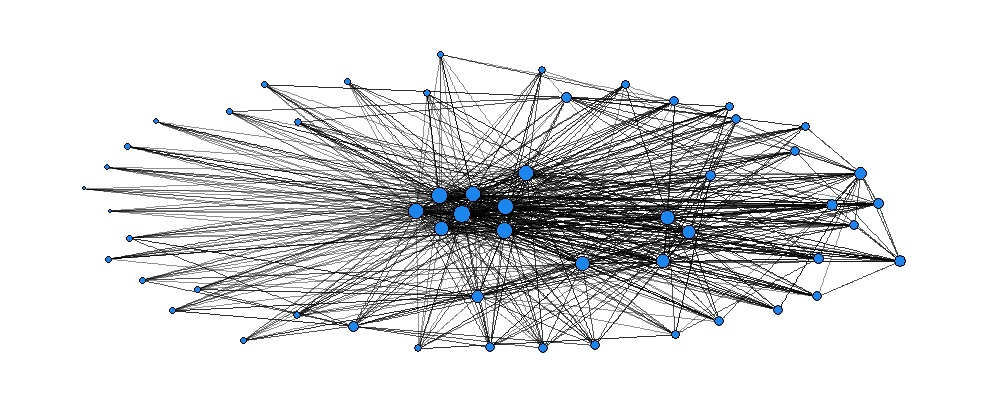
\includegraphics[width=320pt, height=250pt]{./pic/teachers_all_degree.jpg}
    \caption{Sociogram sítě kontaktů mezi učiteli. Velikost uzlů odpovídá počtu jejich vazeb (tj. stupni).}
    \label{fig:100-students}
\end{figure}

\begin{figure}[ht]
    \centering
    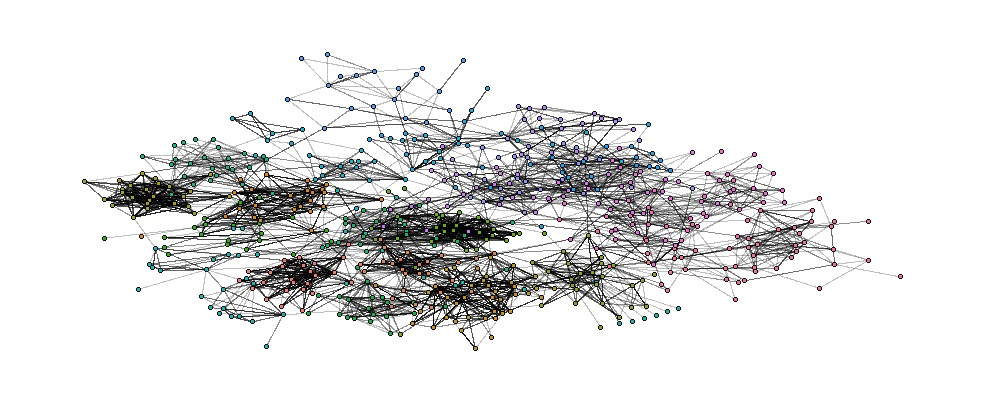
\includegraphics[width=340pt, height=270pt]{./pic/students_all_classes2.jpg}
    \caption{Sociogram sítě kontaktů mezi žáky. Barva uzlů odpovídá jednotlivým školním třídám.}
    \label{fig:100-teachers}
\end{figure}

\section*{Model a simulace}
Pro simulaci dopadů jednotlivých režimových opatření na šíření covid-19 ve škole byl využit agentní epidemiologický model, vyvinutý původně pro simulaci šíření covid-19 ve městě, jak popisuje kapitola 11 tohoto sborníku. Takový model kombinovaný s empiricky získanou sítí kontaktů představuje nejlepší způsob, jak zhodnotit dopad jednotlivých režimových opatření omezení provozu školy. 

Tato opatření se mohou zakládat na dostupné teorii, praktické potřebě a možnostech daného modelu. Zde budou porovnána čtyři různá opatření, která představují jen úzký výběr z celé řady dalších myslitelných opatření v prostředí základních škol (více simulovaných opatření v \cite{Brom2021.06.28.21259628}). Vzhledem k tomu, že během konzumace jídla a pití v jídelně může docházet k výraznému zvýšení virové nálože ve vzduchu (viz např. \cite{Chen_etal2020, eichler2021transmission}), prvním zkoumaným opatřením bude prosté uzavření školní jídelny a společných obědů mezi žáky, modelované jako úplné uzavření vrstvy kontaktů během oběda. Druhým opatřením, které je relativně snadno dostupné, je tzv. homogenizace tříd, neboli zamezení kontaktů mezi žáky napříč rozdílnými školními třídami. V tomto scénáři tak žákům zůstávají pouze ty kontakty, které mají s ostatními z jejich vlastní třídy. Posledním opatřením jsou tzv. rotace, kdy v každém ročníku třída A nejprve má prezenční výuku, zatímco třída B má výuku distanční a každý týden se v tomto schématu střídají. Za účelem zachycení citlivosti jednotlivých opatření na celkový průběh epidemie v populaci je každé opatření simulováno ve čtyřech různých podmínkách odpovídající slabé epidemii (průměrný denní import infekčních jedinců odpovídá 14,6 na 100 tisíc jedinců v celé populaci) až po epidemii silnou (denní import 146 infekčních jedinců na 100 tisíc v populaci).

\section*{Struktura sítě} 

\begin{table}[]
    \centering
    \caption{Struktura sítě kontaktů mezi učiteli}
\begin{tabular}{lccc}
\hline
                 & \multicolumn{3}{c}{vrstva}                                                                      \\ 
                 & \multicolumn{1}{l}{kabinet} & \multicolumn{1}{l}{mimo kabinet} & \multicolumn{1}{l}{mimo školu} \\ \hline
počet uzlů       & 55                          & 55                               & 55                             \\
počet vazeb      & 1122                        & 50                               & 458                            \\
hustota          & 0.378                       & 0.017                            & 0.154                          \\
centralizace     & 0.646                       & 0.136                            & 0.878                          \\
koef. shlukování & 0.505                       & 0                                & 0.251                          \\
prům. vzdálenost & 1.622                       & 3.740                            & 1.846                          \\
diametr          & 2                           & 9                                & 2                              \\ \hline
\label{fig:100-teachers}
\end{tabular}
\end{table}

Co se struktury kontaktů mezi učiteli týče, pozoruhodné jsou dva aspekty. Jednak je celá síť nezanedbatelně centralizovaná, tedy se v ní vyskytuje několik vysoce centrálních učitelů, kolem nichž se koncentruje velké množství kontaktů. Dále pak je také celá síť propojená v jeden celek a to s krátkými vzdálenostmi. To dohromady znamená, že v případě nákazy jednoho z učitelů (obzvláště v případě těch vysoce centrálních) se může nákaza velice rychle rozšířit mezi všechny ostatní učitele. Na propojenosti celé této úrovně sítě se nejvíce podílí kontakty v rámci jednoho kabinetu, kterých je více než dvakrát více než kontaktů v práci mimo kabinet, přičemž se do určité míry překrývají se zbylými typy kontaktů. 

\begin{table}[]
    \centering
    \caption{Struktura sítě kontaktů mezi žáky}
\begin{tabular}{lccccc}
\hline
                 & \multicolumn{5}{c}{vrstva}                                                                                                                           \\ 
                 & \multicolumn{1}{l}{družina} & \multicolumn{1}{l}{lavice} & \multicolumn{1}{l}{mimo školu} & \multicolumn{1}{l}{oběd} & \multicolumn{1}{l}{přestávka} \\ \hline
počet uzlů       & 624                         & 624                        & 624                            & 624                      & 624                           \\
počet vazeb      & 1558                        & 1018                       & 2356                           & 3096                     & 9364                          \\
hustota          & 0.004                       & 0.003                      & 0.006                          & 0.008                    & 0.024                         \\
centralizace     & 0.038                       & 0.009                      & 0.034                          & 0.031                    & 0.035                         \\
koef. shlukování & 0.553                       & 0.235                      & 0.225                          & 0.490                    & 0.663                         \\
prům. vzdálenost & 1.841                       & 3.450                      & 6.017                          & 1.990                    & 4.790                         \\
diametr          & 5                           & 11                         & 14                             & 5                        & 10                            \\ \hline
\label{tab:100-students}
\end{tabular}
\end{table}

Struktura kontaktů mezi žáky se v lecčems liší od struktury kontaktů mezi učiteli. Celá síť je sice také kompletně propojená, zdaleka však není tolik centralizovaná. Na místo toho vykazuje silné shlukování, které je v grafu 2 jasně patrné. Tyto shluky odpovídají jednotlivým školním třídám. Nejvíce kontaktů se odehrává o přestávkách uvnitř tříd, třikrát více než v druhém nejfrekventovanějším případě (obědy). Mezi těmito dvěma druhy kontaktů sice existuje značný překryv, zároveň ale každý typ kontaktů pokrývá i unikátní část sítě, takže prosté omezení jednoho typu kontaktů nemusí vůbec celkovou propojenost sítě zásadním způsobem oslabit. Za zmínku stojí také poměrně velké množství kontaktů jdoucích napříč třídami ve škole (směřujících mezi jednotlivými shluky) a také nemalá proporce i rozprostření kontaktů, které se mezi žáky odehrávají zcela mimo školní prostředí. 

Kombinace propojenosti obou úrovní kontaktů, centralizace úrovně kontaktů mezi učiteli a zároveň jejich pozice propojující obě úrovně prostřednictvím vyučování v různých třídách vystavuje učitele jednak riziku nakažení a zároveň také rychlého přenosu nákazy. 

    
\section*{Simulace opatření} 

\begin{table}[]
    \centering
    \caption{Efekt vybraných simulací na šíření epidemie uvnitř školy}
\begin{tabular}{lcccc}
\hline
                       & \multicolumn{4}{c}{stupeň epidemie} \\ 
                       & slabá   &         &        & silná  \\ \hline
vše otevřeno (výchozí) & 100     & 100     & 100    & 100    \\
omezení obědů          & 61.7    & 66.86   & 66.03  & 68.49  \\
homogenizace tříd      & 67.06   & 68.52   & 71.19  & 74.34  \\
rotace tříd po týdnu   & 18.93   & 21.94   & 22.69  & 24.79  \\
vše zavřeno            & 0       & 0       & 0      & 0      \\ \hline
\label{tab:100-sims}
\end{tabular}
\end{table}

Výsledky simulací jsou shrnuty v tabulce 3. Ze tří simulovaných opatření vychází jako jednoznačně nejefektivnější rotace celých tříd po týdnech. Riziko šíření covid-19 bez dalších zvažovaných opatření by tak mělo na základní škole klesnout o 75-80\%. Efektivita tohoto opatření je o to větší, že není citlivá na míru dodržování podobně jako ostatní režimová opatření (např. větrání nebo ochrana nosu a úst). Jeho další výhodou oproti jiným opatřením je relativně menší zásah do organizace a provozu školy: nevyžaduje významné úpravy rozvrhu a změn pro vyučujících podobně jako například půlení tříd.

Relativně méně efektivní opatření, snižujícími riziko šíření covid-19 o 25-40\%, jsou jednak omezení obědů a také homogenizace třídních kolektivů. Homogenizace tříd zároveň zasahuje významným způsobem do provozu školy, zvláště na 2. stupni. Vyžaduje totiž významné změny rozvrhu (např. odlišnou organizaci jazykových tříd). Omezení obědů znamená významnou komplikaci pro velkou část dětí s ohledem na jejich stravovací návyky a potřeby, především pro děti ze sociálně znevýhodněného prostředí.


\section*{Diskuse} 
Kontaktní sítě v námi studované škole i simulace šíření viru SARS-Cov-2 v této síti společně poukazují na to, jak jsou strukturní vlastnosti dané sítě důležité pro rozsah epidemie. Deskriptivní výsledky ukazují, že především síť kontaktů mezi učiteli je náchylná k rychlému šíření nákazy, protože je hustě propojená a centralizovaná. Nejúčinnějším opatřením jsou rotace celých tříd. Rotace jsou efektivní proto, že významně omezují strukturu kontaktů a zároveň „karanténují“ tu část žáků, která do školy v daném týdnu nechodí. Ačkoliv by se mohlo na první pohled zdát, že docházkou pouze poloviny žáků se infekce sníží o polovinu, efekt je ve skutečnosti výrazně vyšší. Důvodem je to, že se ze sítě kontaktů na čas odejme nejen polovina žáků, ale především jejich kontakty, jejichž proporce je vyšší než polovina a to navíc v hustě propojených vrstvách. Podobný disproporční efekt rotací a celotřídní karantény na snížení rozsahu epidemie dokumentují i další studie \cite{gemmetto2014mitigation, mcgee2021model}. 

Zde uvedená opatření jsou jen úzkým výčtem všech opatření, která lze simulovat na realistické síti kontaktů. Výsledky uvedené výše jsou proto sice validní, nelze je však považovat za vyčerpávající. Širší záběr simulovaných opatření lze nalézt ve výchozí studii \cite{Brom2021.06.28.21259628}. Přesto však i tyto demonstrativní výsledky dokládají užitečnost simulačních modelů pro odhadnutí efektu jednotlivých opatření tam, kde by to jiným způsobem bylo buď nemožné či neetické \cite{squazzoni2020computational}. Model samotný je vždy určitým zjednodušením modelovaného jevu a je proto na místě uvažovat o tom, jak je možné ho v budoucnu rozšířit. Jedním potenciálním rozšířením takového modelu je simulace efektu vakcín se známou účinností pro učitele \cite{mcgee2021model} nebo využít dat o síti kontaktů k explicitnímu modelování dynamiky nejen šíření nákazy, ale i kontaktů samotných \cite{Rao_etal2021}.

Rozšíření modelu, který je představen v této kapitole, se však nemusí omezovat pouze na školní prostředí a nemusí se omezit pouze na covid-19. Za předpokladu dostupnosti dat o relevantních kontaktech lze podobný přístup aplikovat pro simulování různých opatření i v dalších prostředí jakými jsou podniky, úřady nebo ústavy sociální péče. Podobně lze model adaptovat na další infekce za předpokladu, že jsou známy jejich virologické a infektologické vlastnosti. 

Výsledky modelu byly využity Ministerstvem školství, mládeže a tělovýchovy pro nastavení režimových opatření při otevírání škol na jaře 2021. Pro využití na jaře 2021 bylo třeba začít plánovat sběr dat v říjnu a začít sbírat data na začátku listopadu 2020. Model samotný pak byl vyvíjen v průběhu prosince 2020 a ledna 2021. Pro další využití podobných modelů v praxi je tak potřeba čas minimálně v řádu měsíců. To je samozřejmě logisticky i časově poměrně náročné v podmínkách uzavřených škol a do budoucna by proto bylo na místě uvažovat o sběru takových dat preventivně v normálních podmínkách a ve větším počtu různých typů škol. Sběr dat online totiž snižuje návratnost dotazníků a omezení na jednu konkrétní  (byť "typickou") školu je problematický z hlediska reprezentativity.

Sběr dat probíhal na sice vcelku reprezentativní, ale přesto nadprůměrně velké pražské základní škole, z čehož plyne omezená reprezentativita výsledků. Je totiž možné, že se sítě kontaktů mohou mezi školami různých velikostí a typů výrazně lišit. Jakkoliv se data sebraná pro tuto studii podobají datům ze zahraničních studií \cite{gemmetto2014mitigation, mcgee2021model, stehle2011high}, nelze vyloučit, že v případě výrazných a systematických odlišností ve velikosti či organizaci škol se může zkomplikovat zobecnění výsledků pro šíření covid-19 na dalších základních školách. Dalším omezením je to, že se model výhradně zaměřuje na šíření infekce ve škole. Nepočítá tedy nijak s externalitami simulovaných opatření, tj. s tím, jak se omezení provozu škol projeví ve styku žáků a učitelů mimo školní provoz nebo na celkové epidemiologické situaci ve společnosti.




%Na obrázku \ref{fig:100-krivky_pokriv} jsou k vidění dvě osy nebarevné a čtyři křivky barevné.

%\begin{figure}[ht]
 %   \centering
  %  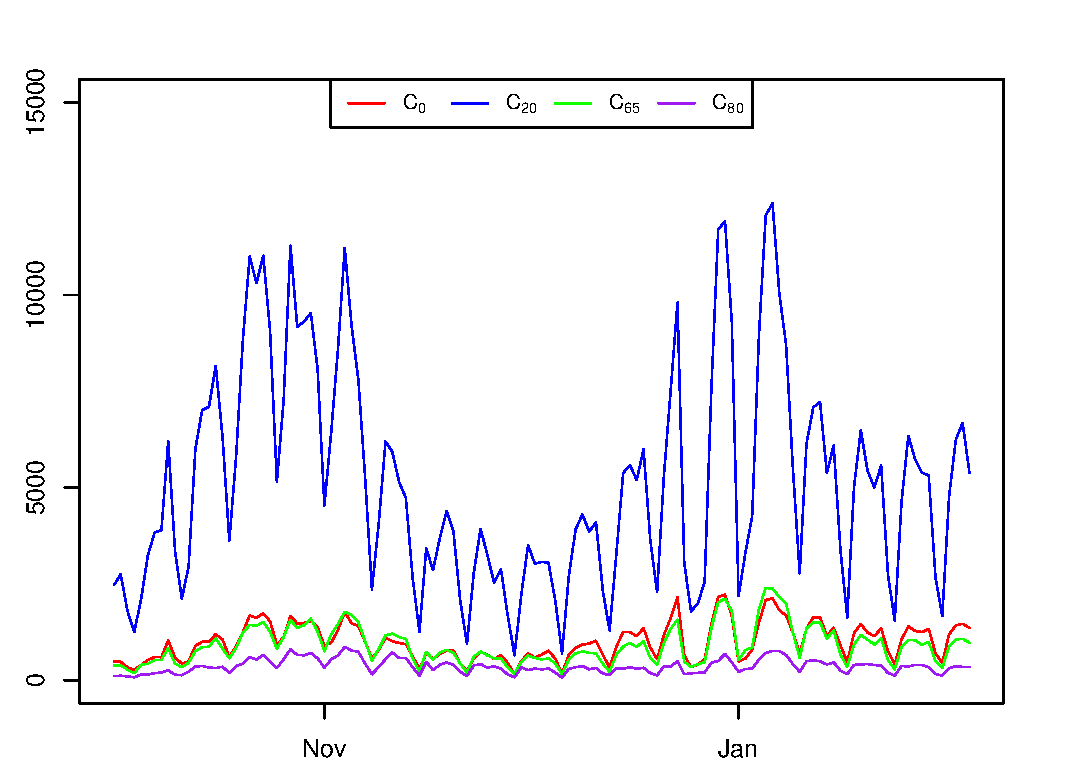
\includegraphics[width=200pt]{./pic/100-C0-80.eps}
   % \caption{Křivky pokřivené}
    %\label{fig:100-krivky_pokriv}
%\end{figure}


%V nálsedujícím testu bude vložena tabulka \ref{tab:100-test}, tabulka jest definována prostředím tabular. Na adrese \url{https://www.overleaf.com/learn/latex/Tables} je dostupný návod jak s tabukami pracovat. Celé prostředí tabular je obaleno blokem table, který umožňuje definovat polohu tabulky na stránce a vložit k tabulce popisek a značku label pro referenci v textu.


%\begin{table}[h]
 %   \centering
  %  \caption{Kódy jednotlivých států použité v číselníku}
%\begin{tabular}{ p{3cm} p{2cm} p{2cm} p{2cm}  }
 %\hline
 %\multicolumn{4}{ c }{Country List} \\
 %\hline
 %Country Name     or Area Name& ISO ALPHA 2 Code &ISO ALPHA 3 Code&ISO numeric Code\\
 %\hline
 %Afghanistan   & AF    &AFG&   004\\
 %Aland Islands&   AX  & ALA   &248\\
 %Albania &AL & ALB&  008\\
 %\hline
%\end{tabular}
    
    %\label{tab:100-test}
%\end{table}

%Odstavce se oddělují prázdným řádkem. Vzhledem k tomu, že text bude převáděn do výsledné grafické podoby, snažte se vyhnout zbytečnému používání \emph{zvýrazněním} a jiným \textbf{grafickým úpravám} textu. Čím více se článek bude blížit čistému textu, tím lépe z hlediska dalšího zpracování příspěvku před finální sazbou. Grafické uspořádání textu po kompilaci je pouze náhledem, nikoli výslednou grafickou podobou.

%V textu je možné - je-li to nutné - používat i matematické vzorce \ref{100-kombin_c}, pro které slouží prostředí equation.

%\begin{equation}
    %\label{100-kombin_c}
    %\binom{n}{k} = \frac{n!}{k!(n-k)!}
%\end{equation}



%Pro zápis do záznamů použivejte syntaxi uvedenou na stránkách: \url{http://bib-it.sourceforge.net/help/fieldsAndEntryTypes.php}